% !TEX TS-program = pdflatex
% !TEX encoding = UTF-8 Unicode

\documentclass[11pt]{article} % use larger type; default would be 10pt

\usepackage[utf8]{inputenc} % set input encoding (not needed with XeLaTeX)
\usepackage{graphicx}
\usepackage{amsmath}
\DeclareGraphicsExtensions{.pdf,.png,.jpg}

%%% Examples of Article customizations
% These packages are optional, depending whether you want the features they provide.
% See the LaTeX Companion or other references for full information.

%%% PAGE DIMENSIONS
\usepackage{geometry} % to change the page dimensions
\geometry{letterpaper} % or letterpaper (US) or a5paper or....
% \geometry{margins=2in} % for example, change the margins to 2 inches all round
% \geometry{landscape} % set up the page for landscape
%   read geometry.pdf for detailed page layout information

\usepackage{graphicx} % support the \includegraphics command and options
\usepackage[parfill]{parskip} % Activate to begin paragraphs with an empty line rather than an indent

%%% PACKAGES
\usepackage{booktabs} % for much better looking tables
\usepackage{array} % for better arrays (eg matrices) in maths
\usepackage{paralist} % very flexible & customisable lists (eg. enumerate/itemize, etc.)
\usepackage{verbatim} % adds environment for commenting out blocks of text & for better verbatim
\usepackage{subfig} % make it possible to include more than one captioned figure/table in a single float
% These packages are all incorporated in the memoir class to one degree or another...

%%% HEADERS & FOOTERS
\usepackage{fancyhdr} % This should be set AFTER setting up the page geometry
\pagestyle{fancy} % options: empty , plain , fancy
\renewcommand{\headrulewidth}{0pt} % customise the layout...
\lhead{}\chead{}\rhead{}
\lfoot{}\cfoot{\thepage}\rfoot{}

%%% SECTION TITLE APPEARANCE
\usepackage{sectsty}
\allsectionsfont{\sffamily\mdseries\upshape} % (See the fntguide.pdf for font help)
% (This matches ConTeXt defaults)

%%% ToC (table of contents) APPEARANCE
\usepackage[nottoc,notlof,notlot]{tocbibind} % Put the bibliography in the ToC
\usepackage[titles,subfigure]{tocloft} % Alter the style of the Table of Contents
\renewcommand{\cftsecfont}{\rmfamily\mdseries\upshape}
\renewcommand{\cftsecpagefont}{\rmfamily\mdseries\upshape} % No bold!

%%% END Article customizations

%%% The "real" document content comes below...

\title{Fast Track – Massively Parallel Programming Techniques Applied to Reinforcement Learning Algorithms. }
\author{Dwight Bell}
%\date{} % Activate to display a given date or no date (if empty),
         % otherwise the current date is printed 

\begin{document}
\maketitle

\section{Reinforcement Learning}

Reinforcement learning is an area within the machine learning field of artificial intelligence.  The goal of reinforcement learning is to produce agents that can successfully choose optimal actions in a problem domain.  The agent learns by observing its current state, taking an action, and receiving a reward.  The reward can be positive, negative or zero and the agent’s goal is to learn how to choose actions to maximize the total reward received over time.

\subsection{Temporal Difference Learning}
The learning approach used here is based on Temporal Difference learning, a model-free approach where the agent does not attempt to build a model of the domain.  Instead, the agent directly learns the present value of future rewards after taking action $a$ from a state $s$, which is represented by the function $Q(s,a)$.  With a good estimate of the  $Q$-function, the agent can determine the best action from a given state by selecting $a$ which maximizes $Q(s,a)$.  The  $Q$-function defines a policy $\pi_Q(s)$ that maps states onto the optimal action according to \eqref{policy}, and the value of a state $V(s)$ according to \eqref{value_fn}.

\begin{equation}
\pi_Q(s)={\operatorname*{argmax}_a}\,Q(s,a)\label{policy}
\end{equation}

\begin{equation}
V_Q(s)={\operatorname*{max}_a}\,Q(s,a)\label{value_fn}
\end{equation}

The $Q$-function can be stated in terms of $R(s,a)$, the expected reward received when taking action $a$ from state $s$, the discount rate ${\gamma}$, and the expected value of the next state, $s^\prime$.

\begin{align}
Q(s,a) &= R(s,a)+\gamma {\operatorname*{E}_{s^\prime}}[V_Q(s^\prime)]\label{value_fn} \\
&= {\operatorname*{E}_{s^\prime}}[R(s,a)+\gamma {\operatorname*{max}_a}Q(s^\prime, a^\prime)] \label{exp_rq}
\end{align}

Equation \eqref{exp_rq} shows that the  $Q$-function can be expressed as the expected value of the reward plus the maximum value of the $Q$-function from the subsequent state.  Whenever an agent takes an action from a state, receives reward and sees the next state, it gets a sample that can be used to improve its estimate of $Q(s,a)$.  The learning rate parameter, $\alpha$, is used to control the degree to which the estimates of $Q(s,a)$ are updated according to equation \eqref{q_update}, where $r$ is the actual reward received.

\begin{equation}
Q(s,a)\gets (1-\alpha)Q(s,a)+\alpha \left(r + \gamma {\operatorname*{max}_{a^\prime}}\,Q(s^\prime, a^\prime)\right) \label{q_update}
\end{equation}

Equation \eqref{q_update} is the basic learning equation for one type of Temporal Difference learning sometimes referred to as  $Q$-learning.

\subsection{Learning the Value Function}
Sometimes the agent knows how to determine the next state after taking an action from the current state.  When this is the case the agent can learn the value function $V(s)$ instead of learning $Q(s,a)$.  The value function defines a policy based on choosing the action that maximizes $V(s^\prime)$, where $s^\prime$ is the known next state after taking action $a$.

\begin{equation}
\pi_V(s)={\operatorname*{argmax}_a}V(s^\prime) \label{policy_v}
\end{equation}

\begin{equation}
V(s)=R(s,a)+\gamma V(s^\prime) \label{v_def}
\end{equation}

Now the agent can use its interactions with the environment to learn the value function using equation \eqref{v_update}.

\begin{equation}
V(s) \gets (1-\alpha )V(s)+\alpha \left(r+\gamma V(s^\prime)\right) \label{v_update}
\end{equation}

Here $\alpha$ is the learning rate and $\gamma$ the discount rate as before.

\subsection{Eligibility Traces}
When learning the $Q$-function, an agent takes an action $a_t$ at time $t$ from a state $s_t$, receives the reward, and observes the next state.  The new information causes the agent to change its estimation of $Q(s_t, a_t)$ using equation \eqref{q_update}.  In principle, the change in the estimated value of $Q(s_t, a_t)$ could then be retroactively used to update the estimated value for $Q(s_{t-1}, a_{t-1})$, the $Q$-value for the state and action that preceded the current one.  Then the additional change in $Q(s_{t-1}, a_{t-1})$ could be used to update $Q(s_{t-2}, a_{t-2})$, etc., propagating the impact of the new information to states and actions further in the past that lead up to the current state.

The impact of a change can be attenuated as it moves further into the past by multiplying by a factor $0<\lambda < 1$.  This method is called TD$(\lambda)$.  To implement TD$(\lambda)$ we first calculate the amount of change, $\delta_t$, and then use that value to update $Q(s_{t-i}, a_{t-i})$ for $i=0,1,2,\dots$

\begin{equation}
\delta_t=\left(r_t+\gamma Q(s_{t+1}, a_{t+1})\right)-Q(s_t, a_t) \label{delta_t}
\end{equation}

\begin{equation}
Q(s_{t-i}, a_{t-i}) \gets Q(s_{t-i}, a_{t-i})+\alpha \lambda^i \gamma^i \delta_t \label{q_update2}
\end{equation}

A computational shortcut uses an $e$-value for each state/action, $e(s,a)$.  When an agent takes an action from a state, the value of $e(s,a)$ is set to $1.0$.  Each time step after that, the $e$-value is decayed by a factor of $\lambda \gamma$ according to equation \eqref{e_update}.

\begin{equation}
e(s,a) \gets \lambda \gamma e(s,a) \label{e_update}
\end{equation}

Then, after calculating $\delta_t$ using equation \eqref{delta_t}, the update rule for all states becomes

\begin{equation}
Q(s,a) \gets Q(s,a) + \alpha e(s,a) \delta_t \label{q_update3}
\end{equation}

\subsection{Other Considerations}
A problem for reinforcement learning in all but the simplest problem domain is the size of the state and action spaces.  Frequently, the size of the state space makes it impossible for the agent to visit all states during the learning process.  The agent must therefore generalize from the portion of the state space it has experienced to estimate the  - or  -functions over the entire domain.  One approach, when the state space is continuous, is to partition the space into a manageable number of cells.  The agent then estimates the function values for each cell. Another approach is to use neural nets to approximate the function of continuous state variables or of an encoding of a high dimensional state.  Each of these approaches is demonstrated in later chapters.

Reinforcement learning can be done in an off-line mode or on-line mode.  Off-line learning means the agent’s rewards received during the learning process do not matter.  The agent’s quality is determined after learning is complete by testing the agent’s optimal policy function and the average reward it will produce.  In on-line learning the agent’s goal is to optimize the reward received while it is learning, a more difficult task.  In this thesis we deal with off-line learning and determine agent quality by pausing the learning process and separately testing the agent’s optimal policy.  Note that sufficiently fast off-line learning methods can be used in an on-line manner by quickly running off-line learning and then selecting the optimal action in the on-line setting.

Reinforcement learning can be applied to a wide variety of problems.  Problem domains for reinforcement learning are classified in a number of ways.  First, problems are classified based on the state information that is available to the agent.  If the agent always sees complete information about the current state of the world the problem the domain is classified as having observable states.  If some information about the current state of the world is hidden from the agent then the problem is called partially observable.  For example, chess is a game with completely observable states, while bridge or poker are domains with partially observable states.  The four problems presented in this thesis have completely observable states.

Another important characteristic of a problem domain is whether the information about the current state that is available to the agent contains all the information that is relevant to predicting the future.  This is referred to as the Markov property and can be stated in probabilistic terms as the future is independent of the past given the present.  All problems in this thesis have the Markov property.  An example of a problem domain that does not have the Markov property is blackjack with a finite deck of cards.  The state may only contain information about the cards currently in play, but the complete history of cards played from the finite deck is relevant to predicting the probabilities of future cards.  Craps is an example of a game that does have the Markov property, as the probabilities in each new game do not depend on prior results.

In general, the agent in a reinforcement learning problem starts with no information about the world it is in, other than the actions it can choose from.  It simply takes an action from the current state and observes the next state that results from that action.  The agent’s only information about how the world works is gathered through its interactions with the problem domain and observing the transitions between states.  This is true for the first three problems in this thesis.  In the last problem, the agent is learning to play a board game through self-play.  The agent does know how the game works.  It is programmed in advance to be able to determine the next state in the game for each of its possible moves from the current state.  It is also programmed with the knowledge of which moves are legal from the current board position.  This approach is common when reinforcement learning is applied to board games.

This brief introduction to reinforcement learning is intended to give a high level view to readers unfamiliar with the topic.  A great source for learning more about reinforcement learning is a textbook by Sutton and Barto ~\cite{Sutton:1998p3536}.


\section{Simple, Discrete Domains}
\subsection{Overview of the Problem}
The first problem is the N-Armed Bandit, a standard problem in reinforcement learning, described by Sutton and Barto (Sutton and Barto, 1998). The N-Armed Bandit problem gets its name from the "one-armed bandit" slot machines in casinos.  The  -armed bandit has more arms, as the name suggests.  The agent must select one of the arms, 'pull' it, and then it receives a variable reward.  The reward is based on a normal distribution that is different for each arm.  The learning problem is to determine which arm has the highest average reward by pulling arms and observing rewards.  The quality of an agent is measured as the percent of times the agent has correctly identified the highest value arm at the end of the learning period.

This problem has only one state and $n$ actions since the agent can choose one of the   arms to pull.  The agent must decide which arm to pull based on the information it has accumulated from previous rewards.  The agent needs to try all arms to get some information about each of them, but should ultimately try to concentrate on the higher-reward arms to find the best one.  The traditional single-agent approach is to keep track of the average reward produced by each arm.  The agent then decides whether to select the arm with the highest reward, or to explore the arms and choose one at random.  The learning parameter, $\epsilon$ , is used to set the probability that a random arm is chosen.  The best arm is chosen with probability $(1-\epsilon)$ .  After the training period, the arm with the highest average reward is the agent’s prediction of the best arm.

TD learning in this domain simplifies to learning $Q(a)$  since there is only one state.  The learning rate, $\alpha$ , is typically set to $1/(n+1)$ where $n$ is the number of times an action has been taken in the past.  This gives the prior estimated value of $Q(a)$ a weight of $n/(n+1)$ and the updated value equals the mean of all observed rewards for action $\alpha$.

Experiments were run using 10-, 100-, and 1000-armed bandits, with qualitatively similar results.  Results shown below are for the 100-armed bandit.

\subsection{Parallel Implementation}
In the parallel implementation for this problem the agents share their information periodically.  The processing is split between periods of learning where each agent operates independently and a sharing period where the information is consolidated from all agents and then shared.  The actual learning and sharing take place on the GPU while the CPU controls the overall process.  The high level division of activities between CPU and GPU is shown in Figure~\ref{fig:seq_diag}.  This diagram shows the basic paradigm I used for the parallel implementation of learning algorithms using the GPU.  It will be updated as the need arises as domains become more complex.

\begin{figure}[hbtp]
\center
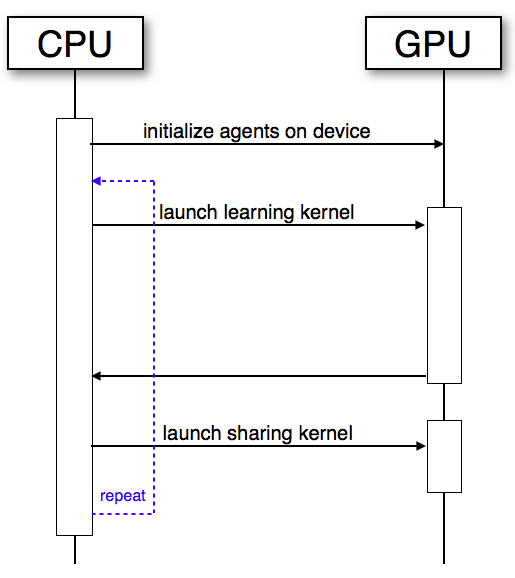
\includegraphics[scale=0.3]{fig01a}
\caption{high-level sequence diagram showing activities on CPU and GPU}
\label{fig:seq_diag}
\end{figure}

\begin{flushleft}

Key learning parameters for the multi-agent parallel approach for the  -Armed Bandit are:

\begin{itemize}
\item
The exploration probability, $\epsilon$ , same as in the single agent algorithm,
\item
the number of parallel agents, and
\item
the frequency of information sharing.
\end{itemize}

\subsection{Sharing and Differentiation}
Each agent keeps track of the number of pulls for each arm and the arm’s average payout.  When sharing occurs an overall count and average is calculated for the block of agents, and then shared back to all agents.  Let $n_i^{[j]}$ be the number of pulls stored by agent $i$ for arm $j$, and $Q_i(j)$ be the value estimated by agent $i$ for arm $j$.  The total values are calculated and each agent is updated based on the following equations for each arm $j$:

\begin{equation}
n_{total}^{[j]}=\sum_in_i^{[j]}
\end{equation}

\begin{equation}
Q_{total}(j)={ {\sum_in_i^{[j]}Q_i(j)} \over {\sum_in_i^{[j]}}}
\end{equation}

For each agent $i$:

\begin{equation}
Q_i(j) \gets Q_{total}(j)
\end{equation}

\begin{equation}
n_i^{[j]} = n_{total}^{[j]}/\mbox{\it number-of-agents} \label{num_pulls}
\end{equation}

Note that in equation \eqref{num_pulls} the number of pulls stored by each agent after sharing is their share of the total number of pulls, not the total number of pulls for the entire block.  This gives less weight to the averages stored by the agent and allows those values to change more dramatically after sharing has occurred.  It also means that the sum of the number of pulls across all agents is equal to the actual total number of pulls.  This is useful when re-calculating the total values at future sharing points.  The result is that some agent's will have their average value for the best arm go down due to the random nature of rewards, perhaps causing another arm to become the best for that agent.  This has the ultimately beneficial effect of causing agents to explore other arms with high average values.

The next time sharing occurs, the block average is recalculated and quality is improved for all agents.  This gives the agents a periodic burst in learning quality at the point of sharing.  The quality may drop between sharing points as the agent’s own values are allowed to vary.  At each sharing point the quality of each agent is restored and actually improves based on the combined information.

\subsection{Results}
Experiments were run with a number of agent differentiation strategies:
\begin{itemize}
\item
partitioning the arms among the agents so when an agent was exploring it would only explore its assigned arm,
\item
random bias given to each agent used when choosing the best arm to pull,
\item
giving some agents in a group a high epsilon value so they would explore with a much greater probability than other agents, and
\item
assigning some agents to randomly choose between the top 2 or top 4 arms when selecting the best arm instead of choosing the actual best arm.
\end{itemize}

There was no dramatic improvement in learning quality from these strategies.  For some, a small improvement in learning quality was more than offset by the increased processing time to implement the more complex logic, resulting in poorer learning as a function of learning time.

Experiments were run for 10-, 100-, and 1000-armed bandits using a single agent and groups of from 4 to 8,192 parallel agents.

The results are broken down into two components to gain a better understanding of the cost and benefits of parallelization.  The first component is learning quality as a function of the number agent-time steps.  An agent time-step is one interaction between an agent and its domain, which equates to one cycle of the learning process executed by one agent.  This will measure the “parallelization penalty” which is the expected reduction in learning quality when a fixed number of agent-time steps are spread over multiple parallel agents, as compared to a single agent operating for all of the time steps.  The penalty occurs because the parallel agents operate independently and only periodically share partial information about their experience.  The single agent is expected to have better learning results, when measured on this basis, since it has complete information available at every time step.

Offsetting the parallel penalty is the speed-up in real time of the parallel implementation.  A fixed number of agent-time steps can run faster if they are executed in parallel, so for a fixed learning period, the parallel approach can execute more agent-time steps than the single agent approach.

The first experiment is for a fixed number of agent-time steps.  Learning is run for the fixed number of agent-time steps and then repeated for 1,024 trials.  Learning quality is calculated as the fraction of the 1,024 trials where the agent correctly identified the bandit with the highest expected payout, which can be determined by inspection.  Measuring learning as a function of agent-time steps gives an understanding of the algorithmic ‘parallel penalty’ from splitting up a fixed number of actions over parallel agents. The results for the 100-armed bandit are shown in Figure~\ref{fig:bandit_steps}.  Learning quality on the y-axis is measured by the probability of correctly identifying the best arm over 1,024 trials.  The blue line with circles is the result for a single agent running on the CPU and the other lines are for different numbers of parallel agents.

\end{flushleft}
\begin{figure}[hbtp]
\center
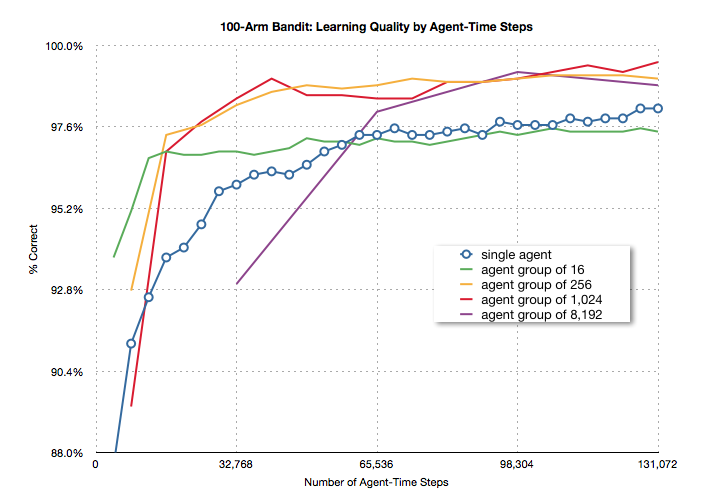
\includegraphics[scale=0.5]{fig02a}
\caption{Learning quality by agent-time steps}
\label{fig:bandit_steps}
\end{figure}

\begin{flushleft}


The results are interesting as there is no clear penalty for the parallel approach, except for agent groups of 16.  When parallel agents numbered 256 or more the parallel implementation actually produced higher quality using a fixed number of agent-time steps.  The difference appears to diminish for extremely large groups as the learning quality drops for 8,192 agents.  The multi-agent advantage is likely coming from more effective exploration due to the lack of complete information.  Each agent in the group makes an independent choice of best arm and the next action to take based on limited information, or perhaps some new unique information it has uncovered but not yet shared, leading to beneficial exploration of the state space.

The next step is to measure learning quality as a function of learning time.  Learning time is the real elapsed time the agent spends interacting with the environment, updating its internal state, and sharing information in the case of parallel agents.  The timing values are for a single learning trial run on the CPU for a single agent, and on the GPU for parallel agents. For parallel runs, the number of time-steps is determined so that the parallel agents took at least as much time as the single agent run for 131,072 time steps.  To get credible quality measurements the results were averaged over 1024 trials for both single agent and parallel agent runs.  Learning quality as a function of learning time is shown in Figure~\ref{fig:bandit_time}.  For the smallest numbers of parallel agents, groups of 16, the parallel implementation on the GPU did poorly compared to the single agent CPU run.  Since the time values were for a single trial, there were only 4 or 16 threads running concurrently on the GPU.  Given the complexity of the calculations and the need to frequently synchronize threads to share information, the poor results are not surprising.  For the larger numbers of parallel agents, with hundreds or thousands of threads, the parallel GPU results clearly surpass the single agent CPU results when learning quality was measured as a function of learning time.

%\end{flushleft}
%\center
%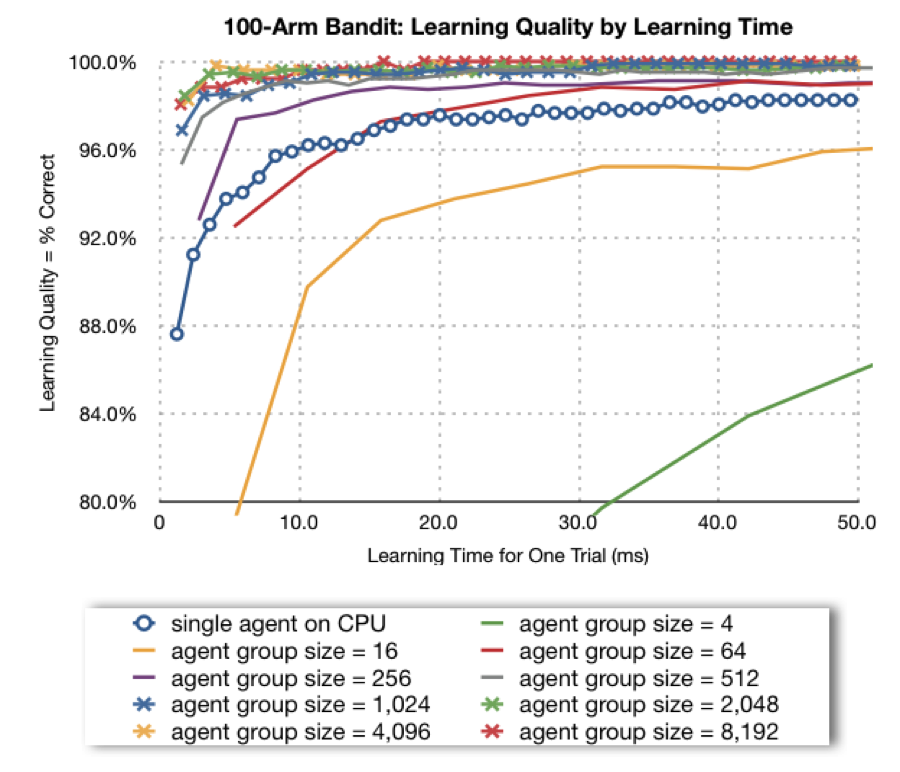
\includegraphics[scale=0.8]{fig04}
%\begin{flushleft}

\end{flushleft}

\begin{figure}[hbtp]
\center
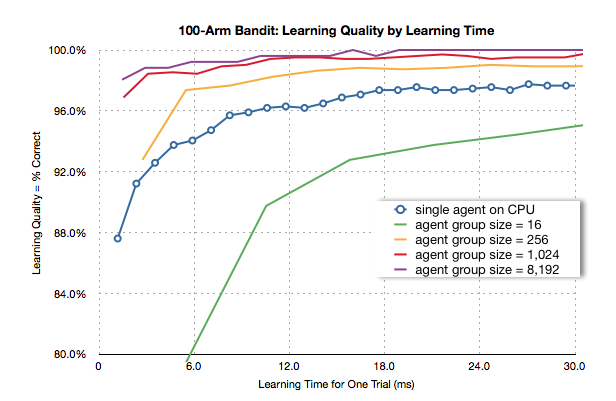
\includegraphics[scale=0.5]{fig03a}
\caption{Learning quality as a function of learning time}
\label{fig:bandit_time}
\end{figure}

\begin{flushleft}


%\end{flushleft}
%\center
%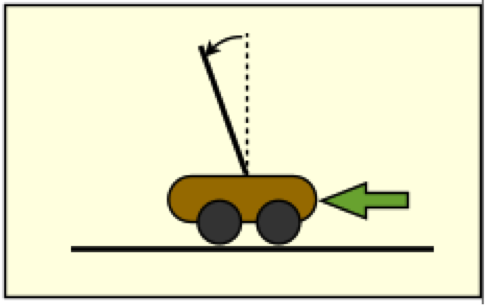
\includegraphics[scale=0.8]{fig06}
%\begin{flushleft}



In summary, the massively parallel approach to the N-armed Bandit problem shows the surprising result that there is no parallel penalty for agent groups of size 64 or larger (Figure~\ref{fig:bandit_steps}).  Splitting a fixed number of agent-state interactions across parallel agents can actually improve the learning quality through more effective exploration.  The parallel results improved further when learning quality is measured as a function of learning time (Figure~\ref{fig:bandit_time}) as the raw speed improvement provided by the GPU allow more agent-time steps to be executed with greater speed in parallel.


\section{Simple, Continuous Domains}
\subsection{Overview of the problem}
The Pole Balancing problem, sometimes referred to as the inverted pendulum, is another canonical problem of reinforcement learning.  The paper “The Pole Balancing Problem, A Benchmark Control Theory Problem” (Brownlee, 2005) contains a detailed description of the standard definition of the problem that was used in this project.  In the Pole Balancing problem, the state consists of a cart on a track with a vertical pole attached to a hinge on the cart.  The goal is to keep the pole balanced within a certain tolerance of the vertical position and to prevent the car from going off either end of the track by applying a fixed force to either end of the car (see Figure~\ref{fig:pole_diag}).  The state of the world consists of four continuous values: the position and velocity of the cart and the angle and angular velocity of the pole.  The agent has no knowledge of how the world works and chooses between two actions: apply the fixed force to the left or to the right.

\end{flushleft}

\begin{figure}[hbtp]
\center
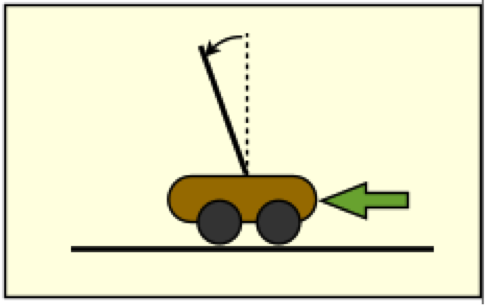
\includegraphics[scale=0.5]{fig06}
\caption{Pole balancing problem}
\label{fig:pole_diag}
\end{figure}

\begin{flushleft}

A reward is introduced to make this a reinforcement learning problem.  The reward is 0 for every time step that the car is on the track and the pole is in the allowable vertical range.  The agent receives a large negative reward if there is a failure due to the car running off the track, or the pole falling beyond the vertical tolerance.  Each trial begins with the state variables being initialized with random values.

This problem poses a new challenge due to the continuous state variables.  There are a number of ways that continuous variables can be handled.  One approach would be to learn a continuous function, $Q(s,a)$, over the continuous domain of the states.  This approach will be used in Chapter ??? .  For this problem we choose to partition the continuous states into a small number of cells.  The position and angle values are partitioned into 3 value ranges.  The cart velocity and angular velocity of the pole are partitioned into two value ranges, positive and negative.  This creates 36 possible discrete states of for the system.  Given the two possible actions, there are a total of 72 state-action values.  This manageable number of state-action values makes it reasonable to try to learn the $Q(s,a)$ function using TD$(\lambda)$ learning.  In this problem the agent attempts to learn the value of $Q(s,a)$ for each state-action pair using eligibility traces.  Eligibility traces should speed learning on this problem as reaching the failure state is intuitively attributable to many prior actions and not just one bad choice.

\subsection{GPU Implementation}
Temporal difference learning with eligibility traces is a complex algorithm to implement on a GPU.  Each agent must maintain a number of values for each state-action pair: the estimated $Q$-value, the eligibility trace, the weight for the $Q$-value that will be used during sharing, and the random bias amount (discussed in next section).   In addition there are random number seeds and stored values for previous state and action.

It is more difficult to monitor the learning process as well.  The agent’s quality cannot be determined by inspection.  It can only be determined by testing, so the learning process must be paused and the agent tested for a statistically significant number of time-steps.  For this problem learning quality is defined as the average time to failure over a trial of 8,192 time-steps.  Testing was done following each sharing phase. 

\subsection{Sharing}
Sharing among agents for this problem is done in a straightforward manner.  After a period of learning, the $Q$-values are averaged over all agents.  The average is done on a weighted basis.  Each agent maintains a weight for each state-action pair.  The weight for agent $i$ is $wgt_i(s,a)$ and it is initialized to a constant value.  During the learning process, the agent weights are updated as follows:

\begin{equation}
wgt_i(s,a) \gets wgt_i(s,a)+\alpha\epsilon_i(s,a)
\end{equation}

During sharing, an average value for all agents for $Q(s,a)$ is calculated based on the following equation:

\begin{equation}
Q_{total}(s,a)={ {\sum_iQ_i(s,a)wgt_i(s,a)} \over {\sum_iwgt_i(s,a)} }
\end{equation}

The value $Q_{total}(s,a)$ is shared with all agents and their weights are reset after sharing to the same constant initial value. 

\begin{equation}
Q_i(s,a) \gets Q_{total}(s,a)
\end{equation}

\begin{equation}
wgt_i(s,a) = \mbox{\it initial-wgt}
\end{equation}

\subsection{Differentiation}
The sharing described above produces identical agents at the start of each learning period.  Differentiation was added to the agents for this problem with beneficial results.  With differentiation, a small random bias amount is added to each agent’s $Q_i(s,a)$ values.  The amount of bias is added after sharing and it decreases over time.  The sharing update rules with differentiation are as follows, where $Rand(-1.0,1.0)$ is a uniform random number over the specified interval, {\it max-bias} is the maximum bias amount and {\it bias-decay-factor} controls the rate of reduction in the maximum bias:

\begin{equation}
Q_i(s,a) \gets Q_{total}(s,a) + Rand(-1.0,1.0) \times \mbox{\it max-bias}
\end{equation}

\begin{equation}
\mbox{\it max-bias} \gets \mbox{\it max-bias} / \mbox{\it bias-decay-factor}
\end{equation}

Randomly biasing the values of $Q(s,a)$ has the most impact on states where $Q(s,LEFT)$ is close to $Q(s,RIGHT)$, i.e. when the values learned so far do not clearly favor one action over the other.  In this situation, the random bias will cause some agents to choose $LEFT$ as the best action and others to choose $RIGHT$, generating new information about both actions from that state.  This, hopefully, leads to identifying one action as clearly the best when the agents pool their information at the next sharing point.  The next section shows the improvement in learning due to differentiation.

\subsection{Results}
Agent quality was measured for this problem as the average time to failure over 8,192 time steps.  Testing is required to determine agent quality as it cannot be determined by inspection.  Each agent is given a random starting state and runs for 8,192 time steps, noting the average time to failure during this period.  The best possible score would be 8,192, which means no failure during the testing period.  Each trial of 8,192 was repeated 1,024 times to get a statistically significant quality measurement.  Doing the quality testing on the GPU sped up the testing since the 1,024 trials can be done in parallel.

The first set of results measure the quality of learning as a function of agent-time steps.  This measurement shows the algorithmic penalty, if any, of the parallel approach.  The algorithmic penalty is the reduction in learning quality due to the fact that agents operating in parallel have less information available to them, after a given number of agent-time steps, than a single agent.  The single agent will have complete information about all actions, rewards, and state transitions, while the parallel agent must wait until a sharing point to gain any information from the experiences of the other agents.

The first graph, Figure\ref{fig:pole_steps}, shows results by agent-time step for varying numbers of parallel agents and compares them to a single agent.  In these runs, there was no differentiation of parallel agents after sharing.  The jump in quality as agents shared information is clearly visible in the graph, but only the smaller agent groups, up to 256 parallel agents, could exceed the single agent learning quality after 262,144 agent-time steps.  The 4,096 agent group, did have an anomalous drop in learning quality at its second sharing point at 262,144 total agent-time steps.  The cause for this was not investigated and the learning quality quickly recovers when the number of time steps per agent increases, as can be seen in Figure ???.

\end{flushleft}

\begin{figure}[hbtp]
\center
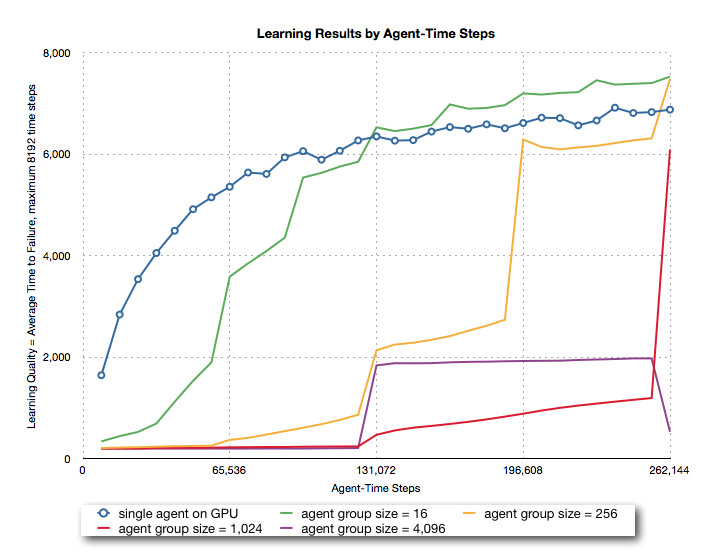
\includegraphics[scale=0.5]{fig07a}
\caption{Learning quality for Pole Balancing as a function of agent-time steps without agent differentiation.}
\label{fig:pole_steps}
\end{figure}

\begin{flushleft}

The frequency of sharing is a learning parameter that is determined separately by agent group size through experimentation.  As agent group size increases, the optimal number of time steps per agent between sharing decreases. 

The next measurements tested learning quality as a function of learning time.  As with the previous problem, learning time is measured based on a single run with the single agent on the CPU or group of parallel agents on the GPU.  The time spent testing the agent is, of course, excluded from the measurement.  The learning quality is then calculated by averaging the learning measurements over 1,024 trials.  The quality of learning with parallel agents is dramatically better than single agent learning for groups of 256 or larger when measured over a learning period of 200ms, as can be seen in Figure~\ref{fig:pole_time}


\end{flushleft}

\begin{figure}[hbtp]
\center
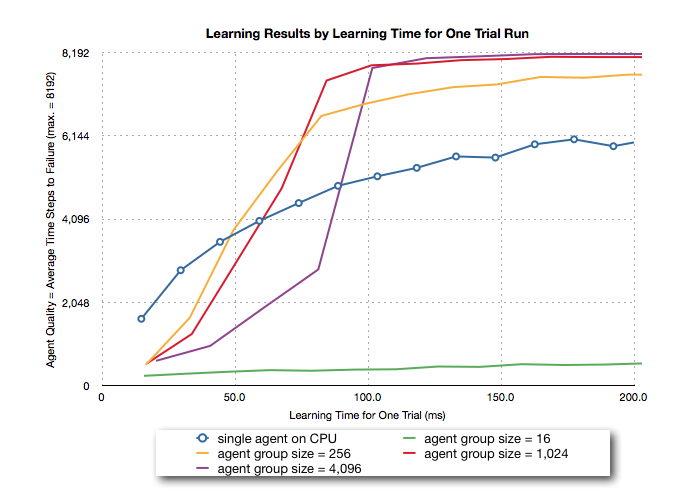
\includegraphics[scale=0.5]{fig08a}
\caption{Learning quality as a function of learning time for Pole Balancing, without agent differentiation.}
\label{fig:pole_time}
\end{figure}

\begin{flushleft}

Agent differentiation is beneficial to parallel learning for the Pole Balancing problem, as mentioned before.  The differentiation for each agent is a small random bias added to the $Q$-values shared with each agent. The amount of random bias was determined by experimentation and decreased exponentially over time.  Differentiation dramatically improves the speed of learning for agent groups of 256 or larger.  Figure~\ref{fig:pole_diff} shows the improvement that occurred during the first 100 ms of learning.  Ultimate quality does not change much because average quality is close to the best possible value of 8,192 and there is no room for improvement.  The final learning quality including the impact of differentiation is shown in Figure~\ref{fig:pole_timediff}, clearly showing the success of the parallel approach.

\end{flushleft}

\begin{figure}[hbtp]
\center
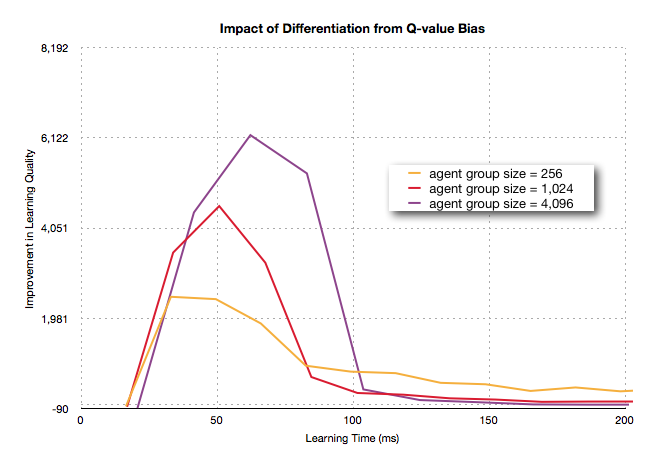
\includegraphics[scale=0.5]{fig09a}
\caption{}
\label{fig:pole_diff}
\end{figure}

\begin{flushleft}

\end{flushleft}

\begin{figure}[hbtp]
\center
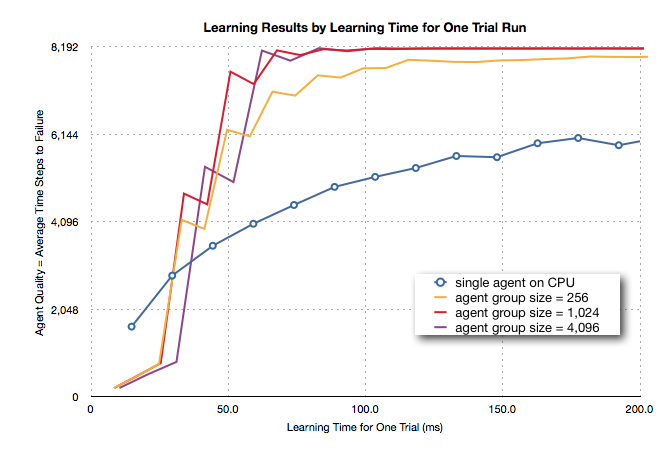
\includegraphics[scale=0.5]{fig10a}
\caption{}
\label{fig:pole_timediff}
\end{figure}

\begin{flushleft}

In summary, the massively parallel approach produces a dramatic improvement in learning quality as a function of the learning time for the Pole Balancing problem (Figure~\ref{fig:pole_timediff}).  This improvement is obtained by using information sharing and agent differentiation with groups of at least 256 parallel agents. 


\section{Learning to Play a Game through Self-Play}
\subsection{Overview of the problem}
The final problem is to learn to play a game through self-play using parallel agents.  The focus is on the ultimate quality of the agent produced, with less emphasis on the speed of learning.  In this problem the agent is pre-programmed with knowledge about how the game works.  That is the agent can determine the next state of the game for any of the actions that are possible from the current state.  It also can determine which actions are legal actions from the current state.  The agent does not know the goal of the game and can not determine in advance what board positions are wins or losses, which must be learned through the reward signal.  The game uses the knight piece from chess on a 5 x 7 chessboard.  The game’s piece movement pattern, number of pieces per side, and board size are variable problem parameters but the results shown here are for knights on a 5 x 7 board and the game starts with the random placement of 5 pieces for each player.  Each player makes a move, as in chess, and a player wins if all opponent’s pieces are captured.  The game has a maximum number of turns and the result is a drawn game when that limit it is reached.

Learning through self-play was advanced by the famous work by Tesauro (Tesauro, 1994) who used TD($\lambda$) and self play to train a program to play backgammon at a master level.  This was dramatic accomplishment and has not yet been duplicated in other domains.  Tesauro points out in his work that it may be the random element that is present in backgammon that drives the learning agent into wide exploration of the state space, enabling high quality learning to take place during self-play.  The random element helps to avoid the problem of converging prematurely to a sub-optimal strategy that can happen with deterministic games.  In those games, the agent may only experience a small fraction of the state space and optimizes for this region only, since by playing itself, it never has to deal with other regions of the state space.

This game is discrete but has a large state/action space.  There are ${35 \choose 5} \times {30 \choose 5}$ possible starting positions with random placement of 5 Xs and 5 Os on a 5 by 7 board.  The total number of game states is even larger since pieces can be removed during the game.  The five knights can move in up to 8 directions each so there may be up to 40 possible actions.  Clearly, there are too many values to learn either $V(s)$ or $Q(s,a)$ for every point and generalization is required.  For this problem I chose to use a neural net to approximate the value function $V(s)$.  The value function can be used by the agent to pick optimal moves with one move look ahead.  The agent loops through possible moves, calculates the board position after each one and selects the move that results in the highest value board position.

\subsection{Neural Net Design}
The neural net must take a description of the board position and output the agent’s estimated value for that board position, $V(s)$.  I coded the board position as two series of binary values for each square on the board.  The first series had the value 1 when player X had a piece on the corresponding square and the second series indicated squares with an O piece.  A single layer of 4 hidden nodes with sigmoid activation is used and the single output node uses sigmoid activation as well.  The number of hidden nodes is a parameter that can vary.  The neural net design is shown Figure ~\ref{fig:neural_net}.

\end{flushleft}
\begin{figure}[hbtp]
\center
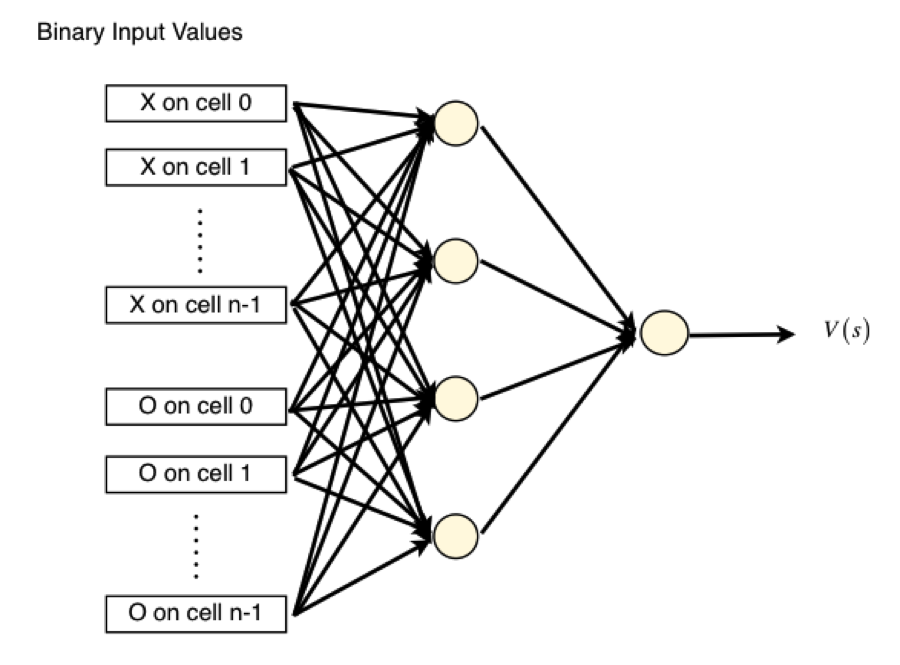
\includegraphics[scale=0.8]{fig11}
\caption{Neural net design for approximating $V(s)$}
\label{fig:neural_net}
\end{figure}
\begin{flushleft}

The learning algorithm for this problem is TD($\lambda$), building on the work done for the previous problems and adapting it to learn the $V(s)$ values.  The weight update rules combine the temporal difference equation for the value function with eligibility traces and back propagation updates for neural net weights.

The basic framework for learning is to have a group of agents learn by playing a set of games against each other.  The relative quality can be gauged by recording the agent’s winning percentage during the learning episodes.  This is shown for an 8-agent group in Figure 23.  The absolute measurement of agent quality requires some outside benchmark or test to be performed.  A benchmark opponent was used to gauge agent quality in Figure 24.  The quality measure is winning percentage calculated as $(wins + draws/2)/games$.

\end{flushleft}
\begin{figure}[hbtp]
\center
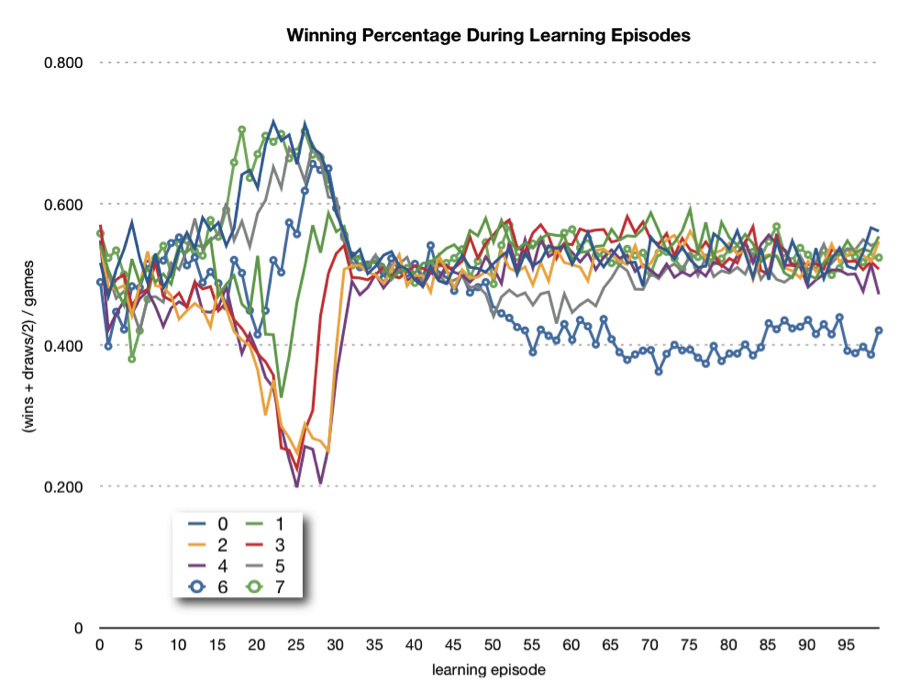
\includegraphics[scale=0.5]{fig12}
\caption{Learning through self-play winning percentage against other agents.}
\label{fig:sp_learning1}
\end{figure}

\begin{figure}[hbtp]
\center
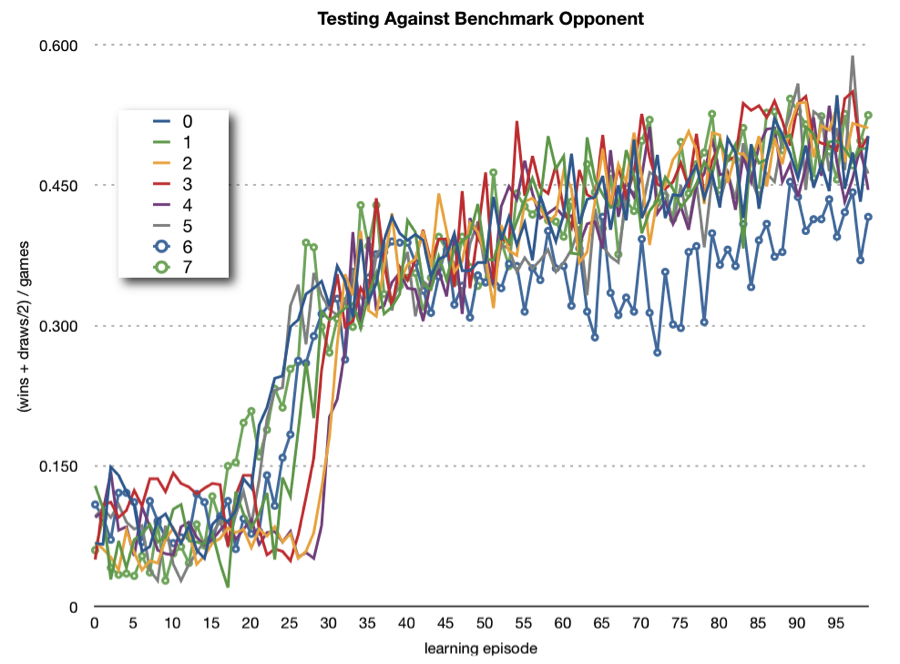
\includegraphics[scale=0.5]{fig13}
\caption{Learning through self-play winning percentage against fixed benchmark opponent.}
\label{fig:sp_learning2}
\end{figure}
\begin{flushleft}


%\subsection{GPU Implementation Issues}
%The algorithm used on this problem is very compute intensive.  For each turn, the agent must look at all possible moves and estimate the value of the next board position by using the neural net estimate $V(s)$.  The GPU implementation uses multiple threads per agent to speed up the neural net calculations and to speed up the weight update calculations that are needed each turn.  Each agent has one thread per board square.  The entire group of threads within an agent will be active during some portions of the processing.  Other times, only a single thread or a smaller group of threads is needed for the calculations.  Thread activity for the choose move function is illustrated in Figure ???.  In that diagram, the green arrows represent active threads and dashed arrows are inactive threads.
%
%\end{flushleft}
%\center
%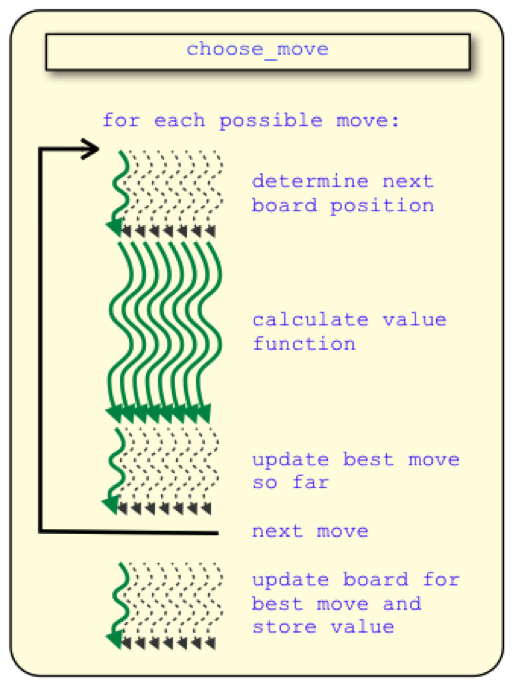
\includegraphics[scale=0.8]{fig14}
%\begin{flushleft}
%
%
%Agents can compete against an opponent in parallel too.  The next diagram, Figure ???, illustrates having $n$ agents compete against one opponent at the same time.
%
%\end{flushleft}
%\center
%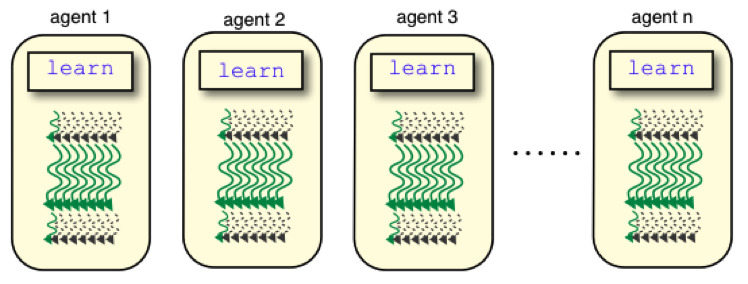
\includegraphics[scale=0.8]{fig15}
%\begin{flushleft}
%
%Having each agent compete against multiple opponents simultaneously increases parallelism further.  This approach requires creating multiple copies of the agent’s weights.  Each copy then competes against a different opponent and updates its own weights.  At the end of an episode of learning, the change in weights across all the copies of an agent is accumulated and the master copy is updated in one batch, illustrated in Figure ???.
%
%\end{flushleft}
%\center
%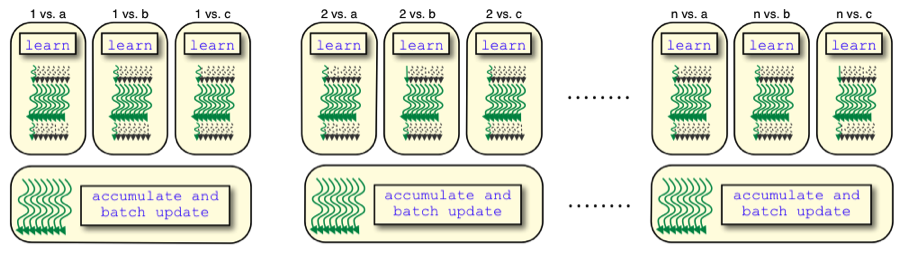
\includegraphics[scale=0.8]{fig16}
%\begin{flushleft}


The processing on both the CPU and GPU is more complicated on this problem than on previous problems.  The GPU is much slower than the CPU for a single agent, but equals CPU speed with 4 agents and is faster for agent groups of 16 or more, as shown in Figure ~\ref{fig:time_per_million}, which displays the learning time for one million turns.

\end{flushleft}
\begin{figure}[hbtp]
\center
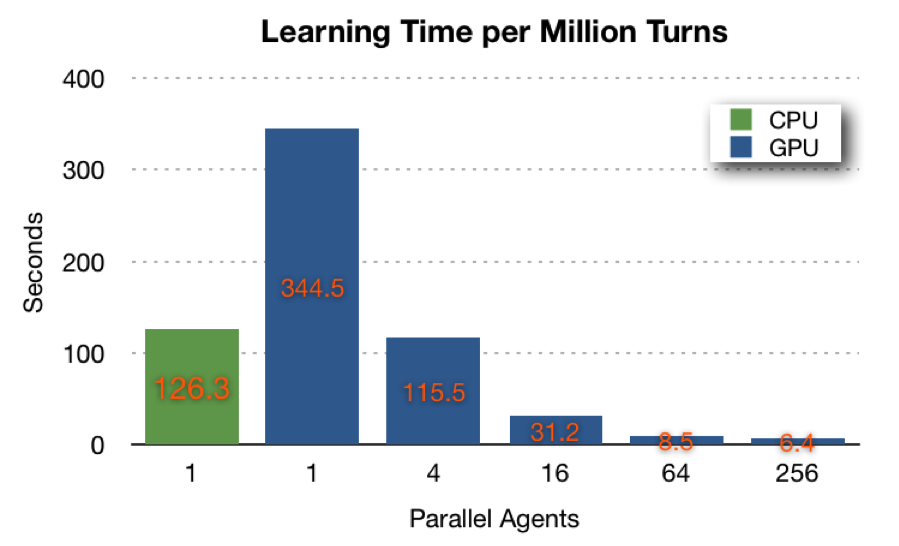
\includegraphics[scale=0.8]{fig17}
\caption{Speed of learning by agent group size.}
\label{fig:time_per_million}
\end{figure}

\begin{flushleft}



\subsection{Replication with Variation and Summary of Results}
There is no direct sharing between parallel agents in this problem.  Indirect sharing happens by agents competing against each other and learning.  If one agent’s quality improves, it becomes a better opponent for the other agents and the other agents should improve as a result as well.

This problem produces a wide variation of agent quality, similar to Mountain Car problem.  Selecting the best agent from a group of parallel agents, based on internal competition between agents or testing against a benchmark opponent, will improve the quality compared to the average result.  Variation in quality can be seen in Figure ~\ref{fig:learn_v_benchmark}, which shows the best, worst, and average agent quality for a group of 64 parallel agents with quality measured against a benchmark opponent.

\end{flushleft}
\begin{figure}[hbtp]
\center
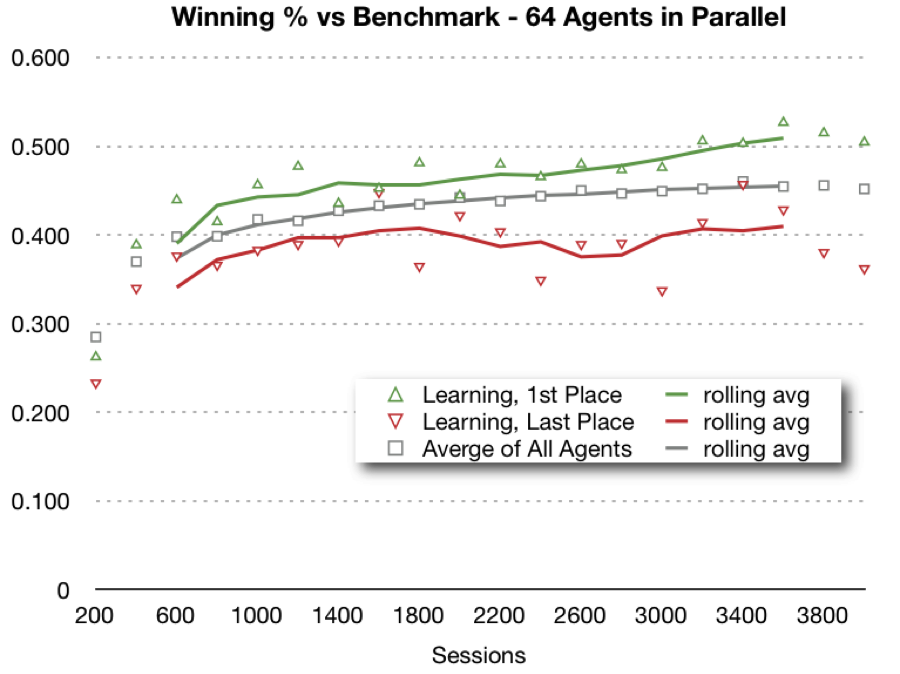
\includegraphics[scale=0.8]{fig18}
\caption{Learning through self-play against benchmark opponent}
\label{fig:learn_v_benchmark}
\end{figure}
\begin{flushleft}


Another technique that works on this problem is the use of selective replication to improve the overall quality of the agent population.  After each learning episode a round-robin competition determines the relative quality of the agents.  The best agents are copied and the worst agents dropped.  In addition, this has a secondary effect of improving the opponents for all agents in the future.  Figure ~\ref{fig:seq_diag_self_play} shows the high-level sequence diagram for CPU and GPU coordination.

\end{flushleft}
\begin{figure}[hbtp]
\center
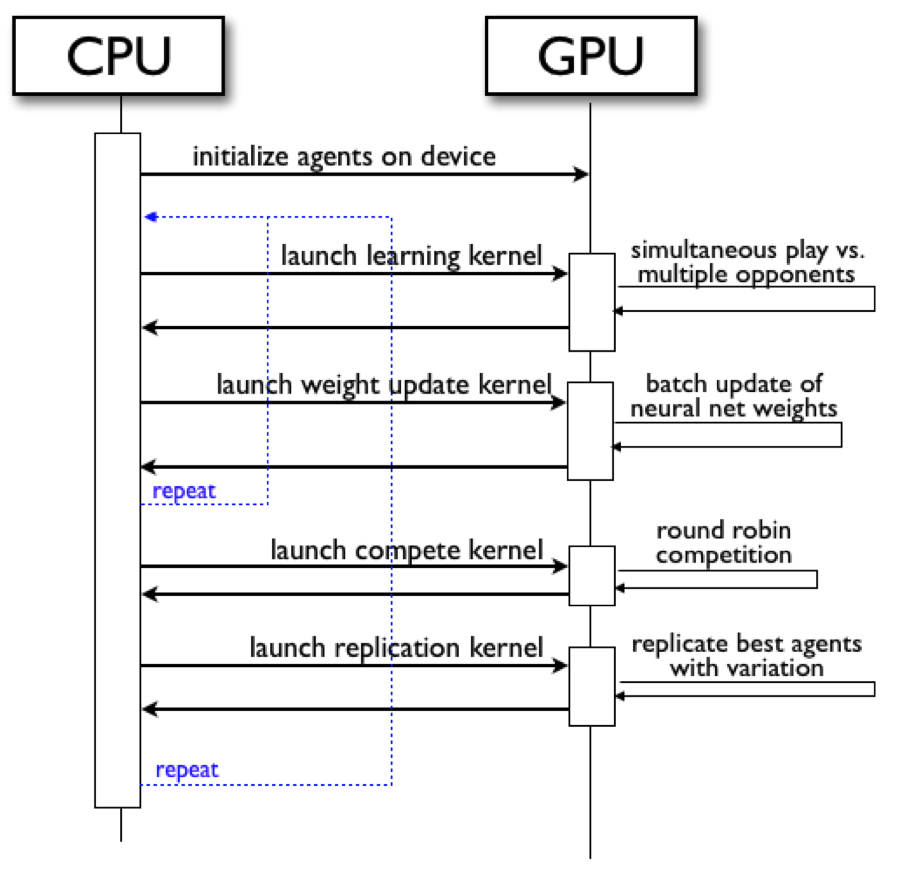
\includegraphics[scale=0.8]{fig19}
\caption{Sequence diagram for learning through self-play in parallel on GPU.}
\label{fig:seq_diag_self_play}
\end{figure}
\begin{flushleft}

The replicated copies of the best agents can include some differentiation.  They can have variation in the learning parameters or slight random bias applied to the neural net weights.  Variation helped the population of agents to continue to improve over a long training session.  The last graph, Figure ~\ref{fig:selection}, shows the typical results when using selective replication with variation with a group of 64 agents.  

\end{flushleft}
\begin{figure}[hbtp]
\center
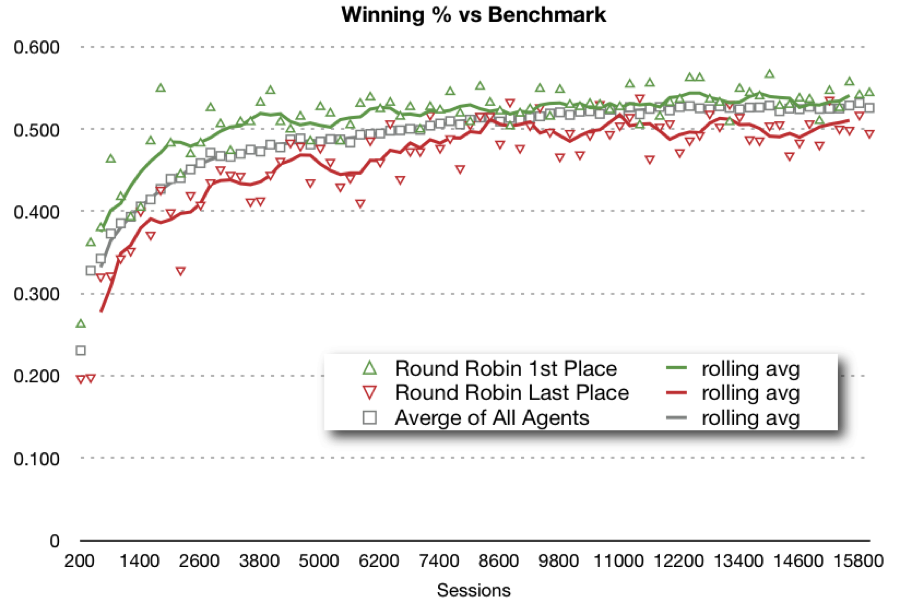
\includegraphics[scale=0.8]{fig20}
\caption{Learning through self-play with selective replication and variation.}
\label{fig:selection}
\end{figure}
\begin{flushleft}


The parallel approach to this problem provides a variety of opponents for agents to learn from.  This can help overcome the problems with self-play using a single agent.  In addition, the evolutionary techniques of selective replication with variation allow the population of agents to continue to improve over time.






\section{Prior Work}

Parallelism techniques have been applied to reinforcement learning in the past.  These applications typically ran on CPUs, but more recently, running on GPUs.  There are also a number of different ways parallelism can be applied.

There are many works that combine multiple agents and reinforcement learning to address a multiagent learning problem.  A Comprehensive Survey of Multiagent Reinforcement Learning ~\cite{Busoniu:2008p4935} describes some of the work in this area.  In contract, this thesis addresses what are traditionally single agent learning problems, and parallelism is used to find the highest quality single agent as fast as possible.  The output of the techniques in this thesis is a single agent even though multiple agents may be used in parallel to find it.

V. Palmer ~\cite{Palmer:2007p4912} used GPU programming to speed up matrix calculations in the Least Squares Policy Iteration algorithm ~\cite{Lagoudakis:2003p4913} applied to a multi-agent cooperative Pole Balancing problem.  The GPU was used to speed up calculations on a fixed set of training data for from 1 to 4 agents where each agent had 20 basis functions.  Here, the parallelism on the GPU was used to get a computational speed up of the policy evaluation and policy improvement steps of the Least Squares Policy Iteration algorithm for each agent.  The implementation and interaction of multiple agents was done on the CPU.  The batch processing using the GPU was compared to a Matlab implementation and found to improve calculation speed for training sets of at least 400 points.  The GPU calculation time grew much slower than the CPU calculation time as the training set increased and also as the number of agents increased.

In this thesis we use the GPU to implement parallelism across multiple agents.  In Palmer’s study, the GPU was used within each agent to speed up that agent’s calculations, but did not attempt to deal with multiple cooperating agents with varying experience and the issues of data communication on the GPU.  Furthermore, the degree of parallelism applied in thesis is much greater, with agent group sizes in hundreds or thousands compared to a maximum of 4 agents in Palmer.

Grounds and Kudenko used a parallel approach with multiple CPUs for three reinforcement learning problems ~\cite{Grounds:2008p3736}.  They parallelized across agents and studied the communication issues between multiple agents.  In their approach, each agent communicated its information to all other agents in a staggered fashion over time.  The agents took turns broadcasting their information to the other agents.  The information communicated was limited to the most important parameters learned by that agent.  The importance of a parameter was determined by how much it changed since the previous communication.  Reducing the quantity of data communicated was necessary due to the relatively slow communication speed between CPUs running on separate machines.  They tested from 1 to 16 agents on Pole Balancing, Mountain Car, and a Grid World problem, and demonstrated increasing quality of learning for a given training time as the number of agents increased.

This thesis differs by running the parallel agents on a single GPU instead of multiple CPUs.  The GPU makes it possible to use thousands of agents while Grounds and Kudenko used a maximum of 16 agents.  Kudenko had to severely limit the quantity of information shared between agents because of the high cost of communication between processes running on different CPUs, which is less of a problem for this thesis.  On the GPU the cost of communication is simply the cost of synchronizing all agents at a sharing point and then calculating and storing values in global memory on the GPU.  Communicating between threads on a single GPU can be less time consuming than communicating between processes on different CPUs.

Kretchmar ~\cite{Kretchmar:2002p3812} applied a parallel approach to the N-armed Bandit problem, which we introduce in Chapter 4.  Kretchmar used from 1 to 10 agents in parallel and the quality of learning was measured as a function of time steps per agent. After each time step, all agents shared information.  Individual agents kept track of their own experience data and that of all other agents separately.  This approach allowed the agents to share just the data from their own experience while still having access to the combined information.  The results showed improved learning quality as the number of agents increased as a function of the number of steps in the learning process.  Measurements were made as a function of action steps per agent, so total actions taken increased as the number of agents was increased.  Results were not timed so the cost of communication between agents was not reflected in the quality measurements.

Kretchmar did not consider the time cost involved with parallel agents and information sharing, and by sharing after every time step the agents had complete information.  In this thesis, time is an important component when measuring of the quality of learning. In this work agents spent most of the time operating independently, agents only share information periodically, and the agents do not have complete information. 

Evolutionary techniques are a natural subject when multiple agents are used.  Evolutionary methods and reinforcement learning are compared in ~\cite{Whiteson:2010p4931}.  In that work the methods are each applied to two learning problems and the problem characteristics which favor reinforcement learning or evolutionary learning are discussed.  Evolutionary methods and reinforcement learning are considered distinct approaches to solving a learning problem.  In this thesis, we combine some evolutionary techniques with the reinforcement learning process implemented by multiple agents, with beneficial results.

The main differences between this thesis and prior work is the use of the GPU to apply massive parallelism to reinforcement learning problems allowing the use of hundreds or thousands of agents. Large numbers of parallel agents are shown to able to improve the reinforcement learning process through a number of techniques.  Empirical measurements are made to demonstrate the improved learning due to information sharing, differentiation, and evolution of hundreds or thousands of agents.


\end{document}
